\documentclass[12pt,fleqn]{article}
\usepackage{./vkCourseML}
\usepackage{vkCourseML}
\usepackage{lipsum}
\usepackage{indentfirst}
\usepackage{graphicx}
\graphicspath{{./figures/}}
\usepackage{tikz}
\usetikzlibrary{positioning,arrows}
\usepackage{amsmath}
\title{Машинное обучение, ФКН ВШЭ\\Семинар №9}
\author{}
\date{13 ноября 2018 г.}

\begin{document}
\maketitle


\section{Градиентный бустинг}

На двух прошедших лекциях обсуждался градиентный бустинг, один из способ построения композиций алгоритмов. Вспомним его основные принципы. Будем искать алгоритм, оптимизирующий некоторую дифференцируемую функцию потерь $L(y, z)$, в виде взвешенной суммы базовых алгоритмов:
\[
    a_N(x)
    =
    \sum_{n = 0}^{N}
        \gamma_n b_n(x).
\]

Идея бустинга заключается в последовательном построении алгоритмов, каждый из которых учитывает ошибки построенной до сих пор композиции:
\[
    \sum_{i = 1}^{\ell}
        L(y_i, a_{N - 1}(x_i) + \gamma_N b_N(x_i))
    \to
    \min_{b_N, \gamma_N}.
\]

После выбора каких-нибудь простых $\gamma_0$ и $b_0(x)$ (например, для задачи регрессии можно положить $\gamma_0 = 1$ и $b_0(x) = \frac 1\ell \sum_{i=1}^l y_i$) все последующие базовые алгоритмы стараются приблизить антиградиент суммы функций потерь, взятый в точках $z = a_{N - 1}(x_i)$:
\[
    s_i
    =
    -
    \left.
    \frac{\partial L}{\partial z}
    \right|_{z = a_{N - 1}(x_i)}.
\]

При этом приближается антиградиент с точки зрения квадратичной функции потерь:
\[
    b_N(x)
    =
    \argmin_{b \in \AA}
        \sum_{i = 1}^{\ell}
            \left(
                b(x_i) - s_i
            \right)^2.
\]

Подбор коэффициентов производится по аналогии с методом наискорейшего спуска:
\[
    \gamma_N = \argmin_{\gamma \in \mathbb{R}}\sum_{i=1}^{\ell} L(y_i, a_{N-1}(x_i) + 
        \gamma b_N (x_i)).
\]

Мы уже знаем, что для квадратичной функции потерь $L(y, z) = 
(y - z)^2$ сдвиги $s_i^*$ выражаются как $s_i^* = y_i - a_N(x_i)$. Посмотрим, 
чему равны сдвиги для других функций потерь.

\begin{vkProblem}
Найдите сдвиги для функции потерь $L(y, z) = |y - z|$.
\end{vkProblem}
\begin{esSolution}

\[
    s_i = - \left. \frac{\partial |y_i - z|}{\partial 
        z} \right|_{z=a_{N-1}(x_i)} = 
    \Bigl. \sign(y_i - z) \Bigr|_{z=a_{N-1}(x_i)} =
    \sign(y_i - a_{N-1}(x_i))
\]

\end{esSolution}

\begin{vkProblem}
Найдите сдвиги для логистической функции потерь \\
$L(y, z) = \log (1 + \exp(-yz))$.
\end{vkProblem}
\begin{esSolution}
Вспомним, что логистическая функция потерь выражается через сигмоиду $\sigma(x) 
= \frac{1}{1 + \exp(-x)}$ следующим образом:

\[
    L(y, z) = \log \left( \frac{1}{\sigma(yz)} \right) = -\log \sigma(yz)
\]

Далее, пользуясь формулой для производной сигмоиды $\sigma'(x) = \sigma(x)(1 - 
\sigma(x))$, получаем

\[
    s_i = \left. \frac{\partial \log \sigma(y_i z)}{\partial z} 
        \right|_{z=a_{N-1}(x_i)} =
    \left. \frac{1}{\sigma(y_i z)} \sigma(y_i z) (1 - \sigma(y_i z)) y_i
        \right|_{z=a_{N-1}(x_i)} =
\]
\[
    = (1-\sigma(y_i a_{N-1}(x_i))) y_i =
    \frac{y_i}{1 + \exp(y_i a_{N-1}(x_i))}.
\]

\end{esSolution}

Теперь посмотрим, как выглядят оптимальные коэффициенты для квадратичной функции потерь:

\begin{vkProblem}
Предположим, что для квадратичной функции потерь $ L$ на очередном шаге бустинга сдвиги для обучения равны $s_i$, и на этих сдвигах был обучен алгоритм $b_N(x)$. Найдите 
оптимальное значение веса алгоритма $\gamma_N$.
\end{vkProblem}
\begin{esSolution}

\[
    \gamma_N = \argmin_{\gamma \in \mathbb{R}} \sum_{i=1}^{\ell} L(y_i, a_{N-1}(x_i) + 
        \gamma b_N (x_i)) =
    \argmin_{\gamma \in \mathbb{R}}\sum_{i=1}^\ell (y_i - (a_{N-1}(x_i) + \gamma b_N (x_i)))^2 =
\]

\[
    = \argmin_{\gamma \in \mathbb{R}}\sum_{i=1}^\ell (s_i - \gamma b_N (x_i)))^2.
\]

Заметим, что функционал является выпуклой функцией относительно $\gamma$, поэтому для нахождения минимума продифференцируем функцию по $\gamma$:

\[
    \frac{\partial \left(\sum_{i=1}^\ell (s_i - \gamma b_N (x_i)))^2 \right) }
        {\partial \gamma} =
    \sum_{i=1}^\ell \frac{\partial (s_i - \gamma b_N (x_i)))^2}{\partial 
    \gamma} =
    \sum_{i=1}^\ell (s_i - \gamma b_N(x_i)) (- b_N(x_i)) =
\]

\[
    = \gamma \sum_{i=1}^\ell b_N(x_i)^2 - \sum_{i=1}^\ell s_i b_N(x_i).
\]

Приравнивая результат к нулю, получаем

\[
    \gamma = \frac{\sum_{i=1}^\ell s_i b_N(x_i)}{\sum_{i=1}^\ell b_N(x_i)^2}.
\]

\end{esSolution}


\section{Градиентный бустинг над деревьями}

С точки зрения разложения на смещение и разброс в ходе обучения каждого нового алгоритма уменьшается смещение композиции, а разброс же остаётся неизменным или увеличивается. Поэтому на практике чаще всего в качестве базовых алгоритмов используются деревья небольшой грубины, обладающие большим смещением, но не склонные к переобучению. Мы знаем, что решающее дерево разбивает все пространство на непересекающиеся области, в каждой из которых его ответ равен константе:
\[
    b_n(x)
    =
    \sum_{j = 1}^{J_n}
        b_{nj}
        [x \in R_j],
\]
где~$j = 1, \dots, J_n$~--- индексы листьев,
$R_j$~--- соответствующие области разбиения,
$b_{nj}$~--- значения в листьях.

Значит, на~$N$-й итерации бустинга композиция обновляется как
\[
    a_N(x)
    =
    a_{N - 1}(x)
    +
    \gamma_N
    \sum_{j = 1}^{J_N}
        b_{Nj}
        [x \in R_j].
\]
Видно, что добавление в композицию одного дерева с~$J_N$ листьями равносильно
добавлению~$J_N$ базовых алгоритмов, представляющих собой предикаты.
Мы можем улучшить качество композиции, подобрав свой коэффициент
при каждом из предикатов:
\[
    \sum_{i = 1}^{\ell}
        L\left(
            y_i,
            a_{N - 1}(x_i)
            +
            \sum_{j = 1}^{J_N}
                \gamma_{Nj}
                [x \in R_j]
        \right)
    \to
    \min_{\{\gamma_{Nj}\}_{j = 1}^{J_N}}.
\]
Поскольку области разбиения~$R_j$ не пересекаются,
данная задача распадается на~$J_N$ независимых подзадач:
\[
    \gamma_{Nj}
    =
    \argmin_\gamma
        \sum_{x_i \in R_j}
            L(y_i, a_{N - 1}(x_i) + \gamma),
    \qquad
    j = 1, \dots, J_N.
\]

Далее на семинаре мы будем сравнивать градиентный бустинг и случайные леса. Для того, чтобы сравнивать сложность построения композиций, получаемых этими методами, нам потребуется решить следующую задачу:

\begin{vkProblem}
Дана выборка из $\ell$ объектов, описываемых $d$ признаками. Приведите временную асимптотику обучения и построения прогнозов для композиции вида $a_N(x) = \sum_{n=0}^N b_n(x)$ над решающими деревьями $b_n$ глубины не более, чем $D$.
\end{vkProblem}
\begin{esSolution}
Для обучения нам необходимо обучить $N$ деревьев, поэтому асимптотика будет $N * T_{tree}$, где $T_{tree}$ - сложность построения одного решающего дерева. При построении одного дерева рассмотрим сложность нахождения оптимального разбиения в одной вершине. Рассмотрим сколько времени тратиться на построение одного уровня в решающем дереве. Обозначим за $\ell^i_j$ - количество объектов из обучающей выборки, доходящих до вершины $j$ на $i$-том уровне (см. Рис. \ref{tree_objects}).

\begin{figure}[!h]
\centering
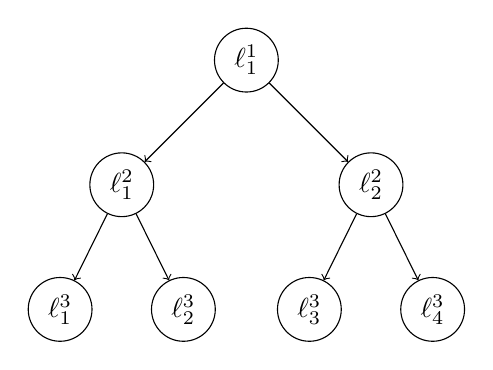
\begin{tikzpicture}[]
\node[circle, draw=black](l11) {$\ell^1_1$};
\node[circle, draw=black, below left = 1cm and 1cm of l11](l21) {$\ell^2_1$};
\node[circle, draw=black, below right = 1cm and 1cm of l11](l22) {$\ell^2_2$};
\node[circle, draw=black, below left = 1cm and 0.2cm of l21](l31) {$\ell^3_1$};
\node[circle, draw=black, below right = 1cm and 0.2cm of l21](l32) {$\ell^3_2$};
\node[circle, draw=black, below left = 1cm and 0.2cm of l22](l33) {$\ell^3_3$};
\node[circle, draw=black, below right = 1cm and 0.2cm of l22](l34) {$\ell^3_4$};
\path[->] (l11) edge (l21);
\path[->] (l11) edge (l22);
\path[->] (l21) edge (l31);
\path[->] (l21) edge (l32);
\path[->] (l22) edge (l33);
\path[->] (l22) edge (l34);
\end{tikzpicture}
\caption{Количество объектов из обучающей выборки, доходящих до каждой из вершин}
\label{tree_objects}
\end{figure}

Нам нужно проверить $d$ признаков по $\ell^i_j - 1$ порогу. Подсчёт метрики качества разбиения занимает $O(\ell^i_j)$ времени. Однако можно реализовать \textit{оптимальный} алгоритм с преподсчитанными статистиками, который для каждого признака сможет вычислить метрику \textit{сразу по всем} $\ell^i_j - 1$ порогам за $O(\ell^i_j)$ времени. Следовательно, для одной вершины требуется $d * O(\ell^i_j) = O(d\ell^i_j)$ времени.

Понятно, что $\ell^1_1 = \ell$, поскольку это самая верхняя вершина. Дальше, для любого $i, j$ верно, что $\ell^i_j = \ell^{i + 1}_{2j - 1} + \ell^{i + 1}_{2j}$ по принципу сохранения стоков-истоков (число объектов, исходящих из одной вершины до её детей, равна числу объектов, входящих в эту вершину). Из этого следует, что в сумме на одном уровне будет всего $\ell$ объектов, $\forall i ~:~ \sum\limits^{2^i}_{j=1} \ell^i_j = \ell$. А значит, на построение одного уровня в решающем дереве нам нужно всего $\sum\limits^{2^i}_{j=1} O(d\ell^i_j) = O(d\ell)$, а уровней всего $D$. Следовательно на построение одного дерева необходимо $T_{tree} = O(Dd\ell)$ времени. У нас $N$ деревьев, следовательно общее время на построение всех деревьев, а значит и на всё обучение: $O(NDd\ell)$

На стадии построения прогноза для объекта $x$ он «пропускается» через дерево от корня к листьям, тем самым проходя путь из не более чем $D$ внутренних вершин, в каждой из которых происходит проверка предиката за константное время. Отсюда имеем асимптотику для построения прогноза композиции — $O(ND)$.

\end{esSolution}

Заметим также, что, поскольку обучение градиентного бустинга является «направленным», то ему требуется меньшее по сравнению со случайным лесом количество базовых алгоритмов для достижения того же качества композиции.

\end{document}
